\documentclass[12pt]{article}
\usepackage[paper=letterpaper,margin=2cm]{geometry}
\usepackage{amsmath,amssymb,amsfonts}
\usepackage{newtxtext,newtxmath}
\usepackage{enumitem}
\usepackage{titling}
\usepackage{subfig,graphicx}
\usepackage[colorlinks=true]{hyperref}
\usepackage{multirow}
\usepackage{listings}
\usepackage[dvipsnames]{xcolor}
\usepackage{float}

\definecolor{codegreen}{rgb}{0,0.6,0}
\definecolor{codegray}{rgb}{0.5,0.5,0.5}
\definecolor{codepurple}{rgb}{0.58,0,0.82}

% BACKGROUND BOX COLORS
\definecolor{bblue}{HTML}{7cc0f3}
\definecolor{bgreen}{HTML}{84b082}
\definecolor{bred}{HTML}{f6908e}
\definecolor{byellow}{HTML}{e0b400}
\definecolor{bmint}{HTML}{00c49a}

% \highlight[<colour>]{<stuff>}
\newcommand{\highlight}[2][yellow]{\mathchoice
  {\colorbox{#1}{$\displaystyle#2$}}
  {\colorbox{#1}{$\textstyle#2$}}
  {\colorbox{#1}{$\scriptstyle#2$}}
  {\colorbox{#1}{$\scriptscriptstyle#2$}}}

\lstdefinestyle{mystyle}{
    commentstyle=\color{codegreen},
    keywordstyle=\color{magenta},
    numberstyle=\tiny\color{codegray},
    stringstyle=\color{codepurple},
    basicstyle=\ttfamily\footnotesize,
    breakatwhitespace=false,
    breaklines=true,
    captionpos=b,
    keepspaces=true,
    numbers=left,
    numbersep=6pt,
    showspaces=false,
    showstringspaces=false,
    showtabs=false,
    tabsize=2
}
\lstset{style=mystyle}

\begin{document}
\begin{center}
\large{Aprendizagem 2023} \\
Homework III -- Group 28 \\
\vskip 0.3cm
Gonçalo Bárias (ist1103124) \& Raquel Braunschweig (ist1102624)\vskip 1cm

\large{\textbf{Part I}: Pen and Paper}\normalsize
\end{center}

\noindent For questions in this group, show your numerical results with 5 decimals or scientific notation. \\
\textit{Hint}: we highly recommend the use of \texttt{numpy} (e.g., \texttt{linalg.pinv} for inverse) or other programmatic
facilities to support the calculus involved in both questions (1) and (2).

\begin{enumerate}[leftmargin=\labelsep]
    \item \textbf{Consider the problem of learning a regression model from 4 bivariate observations} \\

          \vskip -0.2cm
          \textbf{$\left\{\begin{pmatrix} 0.7 \\ -0.3 \end{pmatrix}, \begin{pmatrix} 0.4 \\ 0.5 \end{pmatrix}, \begin{pmatrix} -0.2 \\ 0.8 \end{pmatrix},
          \begin{pmatrix} -0.4 \\ 0.3 \end{pmatrix}\right\}$ with targets $(0.8, 0.6, 0.3, 0.3)$.}

    \begin{enumerate}
        \item \textbf{Given the radial basis function, $\phi_j(x) = \text{exp}\left({ -\frac{\| \mathbf{x} - \boldsymbol{c}_j \|^2}{2} }\right)$ that transforms
              the original space onto a new space characterized by the similarity of the original observations to the following data points
              $\left\{ c_1 = \begin{bmatrix} 0 & 0 \\ \end{bmatrix}^T,\, c_2 = \begin{bmatrix} 1 & -1 \\ \end{bmatrix}^T,\, c_3 = \begin{bmatrix} -1 & 1 \\ \end{bmatrix}^T\right\}$. \\
              Learn the Ridge regression ($l_2$ regularization) using the closed solution with $\lambda = 0.1$.}

              \vskip 0.3cm
              \textbf{Note:} The intermediate values and matrices, in both items of this exercise, show values rounded to 5 decimal places,
              but all intermediate calculations have been carried out without rounding. The values were obtained with the help of \texttt{numpy}
              as suggested in the prompt. The code can be found in the Jupyter notebook \texttt{G028.ipynb}.

              Considering the data points along with the 4 bivariate observations, we can calculate the values of $\phi_1(x), \phi_2(x)$
              and $\phi_3(x)$ for each observation, with $\phi_0(x)$ always being equal to 1.

              \begin{center}
                  \captionsetup{type=table}
                  \begin{tabular}{c|cccc}
                      $x$           & $\phi_0(x)$ & $\phi_1(x)$ & $\phi_2(x)$ & $\phi_3(x)$ \\
                      \hline
                      $(0.7, -0.3)$ & 1           & 0.74826     & 0.74826     & 0.10127     \\
                      $(0.4, 0.5)$  & 1           & 0.81465     & 0.27117     & 0.33121     \\
                      $(-0.2, 0.8)$ & 1           & 0.71177     & 0.09633     & 0.71177     \\
                      $(-0.4, 0.3)$ & 1           & 0.88250     & 0.16122     & 0.65377
                  \end{tabular}
                  \captionof{table}{Value of $\phi_j(x)$ for each observation, $j=0,\dots,3$}
                  \label{ex1a-phi-table}
              \end{center}

              Our goal is to perform a regression where the prediction is given by:
              \begin{equation}\label{ex1a-z-hat}
                  \hat{z}(x, w)
                  = \highlight[bblue]{w_0}\phi_0(x) +
                  \highlight[bred]{w_1}\phi_1(x) +
                  \highlight[bgreen]{w_2}\phi_2(x) +
                  \highlight[byellow]{w_3}\phi_3(x)
              \end{equation}

              Since we want to learn a Ridge regression model, we will need to minimize the following regularized least-squares estimator:
              \begin{equation}\label{ex1a-least-squares}
                  E(w) = \frac{1}{2} \sum_{i = 1}^{N} (z_i - w^T \cdot x_i)^2 + \frac{\lambda}{2} \| w \|_{2}^2
              \end{equation}

              To minimize \eqref{ex1a-least-squares}, we set its gradient equal to 0 and obtain the closed-form solution with $\lambda = 0.1$ in equation \eqref{ex1a-ridge}.
              In the equation, we have that $\Phi$ is the matrix after applying $\phi_j(x)$ to the observations (Table \ref{ex1a-phi-table}) and $z$ is the vector
              of targets for the observations, $z = \begin{bmatrix}0.8 & 0.6 & 0.3 & 0.3\end{bmatrix}^T$.

              \vskip -0.2cm
              \begin{equation}\label{ex1a-ridge}
                  \nabla E(w) = 0 \;\Leftrightarrow\; w = \left(\Phi^T \Phi + \lambda I\right)^{-1} \cdot \Phi^T z
                  \;\Leftrightarrow\; w = \left(\Phi^T \Phi + 0.1 I\right)^{-1} \cdot \Phi^T z
              \end{equation}

              \vskip -0.2cm
              $$
                  \Phi = \begin{bmatrix}
                      1.00000 & 0.74826 & 0.74826 & 0.10127 \\
                      1.00000 & 0.81465 & 0.27117 & 0.33121 \\
                      1.00000 & 0.71177 & 0.09633 & 0.71177 \\
                      1.00000 & 0.88250 & 0.16122 & 0.65377
                  \end{bmatrix}
                  \quad
                  \quad
                  \Phi^T = \begin{bmatrix}
                      1.00000 & 1.00000 & 1.00000 & 1.00000 \\
                      0.74826 & 0.81465 & 0.71177 & 0.88250 \\
                      0.74826 & 0.27117 & 0.09633 & 0.16122 \\
                      0.10127 & 0.33121 & 0.71177 & 0.65377
                  \end{bmatrix}
              $$

              \textbf{Therefore}, we can then calculate the remaining values, until we get the vector $w$:

              $$
                  \begin{aligned}
                      \Phi^T \Phi                                          & = \begin{bmatrix}
                                                                                   4.00000 & 3.15718 & 1.27698 & 1.79802 \\
                                                                                   3.15718 & 2.50897 & 0.99165 & 1.42916 \\
                                                                                   1.27698 & 0.99165 & 0.66870 & 0.33955 \\
                                                                                   1.79802 & 1.42917 & 0.33956 & 1.05399
                                                                               \end{bmatrix}                                                            \\
                      \Phi^T \Phi + \highlight[bmint]{0.1} I               & = \begin{bmatrix}
                                                                                  \highlight[bmint]{4.10000}  & 3.15718 & 1.27698 & 1.79802 \\
                                                                                   3.15718 & \highlight[bmint]{2.60897} & 0.99165 & 1.42917 \\
                                                                                   1.27698 & 0.99165 & \highlight[bmint]{0.76870} & 0.33956 \\
                                                                                   1.79802 & 1.42917 & 0.33956 & \highlight[bmint]{1.15399}
                                                                               \end{bmatrix}                                                            \\
                      \left(\Phi^T \Phi + 0.1 I\right) ^ {-1}              & = \begin{bmatrix}
                                                                                   4.54826  & -3.77682 & -1.86117 & -1.86155 \\
                                                                                   -3.77682 & 5.98285  & -0.88543 & -1.26432 \\
                                                                                   -1.86117 & -0.88543 & 4.33276  & 2.72156  \\
                                                                                   -1.86155 & -1.26432 & 2.72156  & 4.53204
                                                                               \end{bmatrix}                                                            \\
                      \left(\Phi^T \Phi + 0.1 I\right) ^ {-1} \cdot \Phi^T & = \begin{bmatrix}
                                                                                   0.14105  & 0.35022  & 0.35575  & -0.30185 \\
                                                                                   -0.09064 & 0.43823  & -0.50361 & 0.53370  \\
                                                                                   0.99394  & -0.50615 & -0.13690 & -0.16477 \\
                                                                                   -0.31222 & -0.65246 & 0.72647  & 0.42436
                                                                               \end{bmatrix}                                                            \\
                      w = \left(\Phi^T \Phi + 0.1 I\right) ^ {-1} \cdot \Phi^T z & = \begin{bmatrix}
                                                                                         \highlight[bblue]{0.33914} & \highlight[bred]{0.19945} &
                                                                                         \highlight[bgreen]{0.40096} & \highlight[byellow]{-0.29600}
                                                                                     \end{bmatrix}^T
                  \end{aligned}
              $$

              Having calculated the vector $w$, we now know the values of each weight in the regression:

              $$
                  \begin{array}{cccc}
                      \highlight[bblue]{w_0 = 0.33914}  &
                      \highlight[bred]{w_1 = 0.19945}   &
                      \highlight[bgreen]{w_2 = 0.40096} &
                      \highlight[byellow]{w_3 = -0.29600}
                  \end{array}
              $$

              \textbf{Finally}, replacing them in \eqref{ex1a-z-hat} gives us the regression expression:

              \begin{equation}\label{ex1a-final-z-hat}
                  \hat{z}(x, w)
                  = 0.33914 + 0.19945\,\phi_1(x) +
                  0.40096\,\phi_2(x) - 0.29600\,\phi_3(x)
              \end{equation}

        \item \textbf{Compute the training RMSE for the learnt regression.}

              \vskip 0.3cm
              The RMSE (Root Mean Square Error) is given by:

              \begin{equation}\label{ex1b-rmse}
                  \text{RMSE} = \sqrt{\frac{1}{N} \sum_{i = 1}^{N} (z_i - \hat{z}_i)^2}
              \end{equation}

              Here we have $N = 4$, because 4 is the number of samples in the dataset, $z_i$ is the true label for the $i$-th sample and $\hat{z}_i$
              is the predicted label for the $i$-th sample.

              Using \eqref{ex1a-final-z-hat} from the previous item, we can determine $\hat{z}$ for the 4 observations:

              $$
                \Phi = \begin{bmatrix}
                      1.00000 & 0.74826 & 0.74826 & 0.10127 \\
                      1.00000 & 0.81465 & 0.27117 & 0.33121 \\
                      1.00000 & 0.71177 & 0.09633 & 0.71177 \\
                      1.00000 & 0.88250 & 0.16122 & 0.65377
                    \end{bmatrix} \,
                \land \,
                w = \begin{bmatrix}{}
                      \highlight[bblue]{0.33914}  \\
                      \highlight[bred]{0.19945}   \\
                      \highlight[bgreen]{0.40096} \\
                      \highlight[byellow]{-0.29600}
                    \end{bmatrix} \,
               \Rightarrow \,
               \hat{z} = \Phi w = \begin{bmatrix}{}
                                   0.75844 \\
                                   0.51232 \\
                                   0.30905 \\
                                   0.38629
                               \end{bmatrix}
              $$

              \textbf{Finally}, we can take $z = \begin{bmatrix}0.8 & 0.6 & 0.3 & 0.3\end{bmatrix}^T$ along with $\hat{z}$ and calculate RMSE, using \eqref{ex1b-rmse}:
              $$
                  \text{RMSE} = \sqrt{\frac{1}{4} \times \sum_{i = 1}^{4} (z_i - \hat{z}_i)^2} = \sqrt{\frac{1}{4} \times 0.01694} = \mathbf{0.06508}
              $$
    \end{enumerate}

    \item \textbf{Consider a MLP classifier of three outcomes - A, B and C - characterized by the following weights and activation function for every unit:} \\

          \begin{center}
              \vskip -0.3cm
              $\text{W}^{[1]} = \begin{pmatrix} 1 & 1 & 1 & 1 \\ 1 & 1 & 2 & 1 \\ 1 & 1 & 1 & 1\end{pmatrix},\; \text{b}^{[1]} = \begin{pmatrix} 1 \\ 1 \\ 1 \end{pmatrix},\;
              \text{W}^{[2]} = \begin{pmatrix} 1 & 4 & 1 \\ 1 & 1 & 1 \end{pmatrix},\; \text{b}^{[2]} = \begin{pmatrix} 1 \\ 1 \end{pmatrix},\;
              \text{W}^{[3]} = \begin{pmatrix} 1 & 1 \\ 3 & 1 \\ 1 & 1\end{pmatrix},\; \text{b}^{[3]} = \begin{pmatrix} 1 \\ 1 \\ 1 \end{pmatrix}$ \\
          \end{center}

          \[ f\left(x\right) = \frac{{e^{0.5x - 2} - e^{-0.5x + 2}}}{{e^{0.5x - 2} + e^{-0.5x + 2}}} = \tanh\left(0.5x - 2\right) \] \\

          \vskip -0.5cm
          \textbf{We also have the squared error loss $\frac{1}{2} \|\mathbf{z} - \hat{\mathbf{z}}\|^{2}_{2}$. Perform one batch gradient descent update (with learning rate $\eta = 0.1$) for training
          obvervations $x_1 = \begin{bmatrix} 1 & 1 & 1 & 1 \\ \end{bmatrix}^T$ and $x_2 = \begin{bmatrix} 1 & 0 & 0 & -1 \\ \end{bmatrix}^T$ with targets B and A,
          respectively.}

          \vskip 0.3cm
          \textbf{Note:} To help with the calculations and as suggested in the prompt, we used \texttt{numpy}.
          The code can be found in the Jupyter notebook \texttt{G028.ipynb}.

          To begin, we initiate the process with the \textbf{forward pass}. Below are the key equations for this step:

          \begin{align*}
              \mathbf{z}^{[n]} = \mathbf{W}^{[n]} \cdot \mathbf{x}^{[n-1]} + \mathbf{b}^{[n]} & \qquad\qquad
              \mathbf{x}^{[n]} = f\left(\mathbf{z}^{[n]}\right)
          \end{align*}

          We will start with $x_1$:
            \begingroup
            \allowdisplaybreaks
            \begin{align*}
                z^{[1]}_1 &= {W}^{[1]} \cdot {x}^{[0]}_1 + {b}^{[1]} = \begin{pmatrix} 1 & 1 & 1 & 1 \\ 1 & 1 & 2 & 1 \\ 1 & 1 & 1 & 1\end{pmatrix} \cdot  \begin{pmatrix} 1 \\ 1 \\ 1 \\ 1 \end{pmatrix} +
                \begin{pmatrix} 1 \\ 1 \\ 1\end{pmatrix} = \begin{pmatrix} 5 \\ 6 \\ 5\end{pmatrix} \\
                {x}^{[1]}_1 &= f\left({z}^{[1]}_1\right) \approx \begin{pmatrix} 0.46212 \\ 0.76159 \\ 0.46212\end{pmatrix} \\
                z^{[2]}_1 &= {W}^{[2]} \cdot {x}^{[1]}_1 + {b}^{[2]} = \begin{pmatrix} 1 & 4 & 1 \\ 1 & 1 & 1\end{pmatrix} \cdot \begin{pmatrix} 0.46212 \\ 0.76159 \\ 0.46212 \end{pmatrix} +
                \begin{pmatrix} 1 \\ 1\end{pmatrix} \approx \begin{pmatrix} 4.97061 \\ 2.68583\end{pmatrix} \\
                {x}^{[2]}_1 &= f\left({z}^{[2]}_1\right) \approx \begin{pmatrix} 0.45048 \\ -0.57642\end{pmatrix} \\
                z^{[3]}_1 &= {W}^{[3]} \cdot {x}^{[2]}_1 + {b}^{[3]} = \begin{pmatrix} 1 & 1 \\ 3 & 1 \\ 1 & 1\end{pmatrix} \cdot  \begin{pmatrix} 0.45048 \\ -0.57642\end{pmatrix} +
                \begin{pmatrix} 1 \\ 1 \\ 1\end{pmatrix} \approx \begin{pmatrix} 0.87406 \\ 1.77503 \\ 0.87406\end{pmatrix} \\
                {x}^{[3]}_1 &= f\left({z}^{[3]}_1\right) \approx \begin{pmatrix} -0.9159 \\ -0.80494 \\ -0.9159\end{pmatrix}
            \end{align*}
            \endgroup

          \vskip -0.2cm
          Next in line is $x_2$:
            \begingroup
            \allowdisplaybreaks
            \begin{align*}
                z^{[1]}_2 &= {W}^{[1]} \cdot {x}^{[0]}_2 + {b}^{[1]} = \begin{pmatrix} 1 & 1 & 1 & 1 \\ 1 & 1 & 2 & 1 \\ 1 & 1 & 1 & 1\end{pmatrix} \cdot  \begin{pmatrix} 1 \\ 0 \\ 0 \\ -1 \end{pmatrix} +
                \begin{pmatrix} 1 \\ 1 \\ 1\end{pmatrix} = \begin{pmatrix} 1 \\ 1 \\ 1\end{pmatrix} \\
                {x}^{[1]}_2 &= f\left({z}^{[1]}_2\right) \approx \begin{pmatrix} -0.90515 \\ -0.90515 \\ -0.90515\end{pmatrix} \\
                z^{[2]}_2 &= {W}^{[2]} \cdot {x}^{[1]}_2 + {b}^{[2]} = \begin{pmatrix} 1 & 4 & 1 \\ 1 & 1 & 1\end{pmatrix} \cdot  \begin{pmatrix} -0.90515 \\ -0.90515 \\ -0.90515 \end{pmatrix} +
                \begin{pmatrix} 1 \\ 1\end{pmatrix} \approx \begin{pmatrix} -4.43089 \\ -1.71544\end{pmatrix} \\
                {x}^{[2]}_2 &= f\left({z}^{[2]}_2\right) \approx \begin{pmatrix} -0.99956 \\ -0.99343\end{pmatrix} \\
                z^{[3]}_2 &= {W}^{[3]} \cdot {x}^{[2]}_2 + {b}^{[3]} = \begin{pmatrix} 1 & 1 \\ 3 & 1 \\ 1 & 1\end{pmatrix} \cdot  \begin{pmatrix} -0.99956 \\ -0.99343\end{pmatrix} +
                \begin{pmatrix} 1 \\ 1 \\ 1\end{pmatrix} \approx \begin{pmatrix} -0.993 \\ -2.99212 \\ -0.993\end{pmatrix} \\
                {x}^{[3]}_2 &= f\left({z}^{[3]}_2\right) \approx \begin{pmatrix} -0.98652 \\ -0.99816 \\ -0.98652\end{pmatrix}
            \end{align*}
            \endgroup

          Let's initiate the \textbf{backpropagation} process. To do this, we first need to take into account the loss function, which, as per the prompt, is defined as follows:

          \begin{equation}\label{ex2-loss}
            \mathcal{L} = \frac{1}{2} \|\mathbf{z} - \hat{\mathbf{z}}\|^{2}_{2} = \frac{1}{2} \left(\mathbf{t} - {\mathbf{o}}\right)^{2}
          \end{equation}

          The next step involves computing its derivative:

          \begin{equation}
            \frac{d\mathcal{L}}{dW^{[p]}} = \sum_{i=1}^{2} \left(\frac{d\mathcal{L}}{dx^{[p]}_i} \circ \frac{dx^{[p]}_i}{dz^{[p]}_i} \cdot \frac{dz^{[p]}_i}{dW^{[p]}} \right)
          \end{equation}

          This can be broken down into:

          \vskip -0.3cm
          \begin{align*}
              \frac{d\mathcal{L}}{dx^{[p]}_i} \circ \frac{dx^{[p]}_i}{dz^{[p]}_i} = \delta^{[p]}_i & \qquad\qquad
              \frac{dz^{[p]}_i}{dW^{[p]}} = \left(x^{[p-1]}_i\right)^{T}
          \end{align*}

          \textbf{Therefore,} the derivative of the loss fuction is given by:

          \begin{equation}\label{ex2-derivate-loss-smiplified}
            \frac{d\mathcal{L}}{dW^{[p]}} = \sum_{i=1}^{2} \left(\delta^{[p]}_i \cdot \left(x^{[p-1]}_i\right)^{T} \right)
          \end{equation}

          When computing \(\delta\), we can split it into two separate cases: if it is in the last layer \eqref{ex2-deltalastlayer}, or in non-external layers \eqref{ex2-deltanotlastlayer}:

          \begin{equation}\label{ex2-deltalastlayer}
              \delta^{[p]}_i = \left(x^{[p]}_i - z_i\right) \circ \text{sech}^{2}\left(0.5 \times z^{[p]}_i - 2\right) \times 0.5
          \end{equation}

          \begin{equation}\label{ex2-deltanotlastlayer}
              \delta^{[p]}_i = \left(W^{[p+1]^{T}} \cdot \delta^{[p+1]}_i\right) \circ \text{sech}^{2}\left(0.5 \times z^{[p]}_i - 2\right) \times 0.5
          \end{equation}

          \textbf{Since,} the \texttt{tanh} function has a codomain of $]-1,1[$ and since the targets for $x_1$ and $x_2$ are B and A, respectively, we can conclude that:

          \vskip -0.3cm
          \[
              \begin{array}{cc}
                  z_1 = \begin{bmatrix} -1 & 1 & -1\end{bmatrix}^T & \qquad
                  z_2 = \begin{bmatrix} 1 & -1 & -1\end{bmatrix}^T
              \end{array}
          \]

        \textbf{Now,} we have all we need to compute the values for the deltas, $\delta$, by replacing the equation on \eqref{ex2-deltalastlayer} for $p=3$,
        and \eqref{ex2-deltanotlastlayer} for any $p \neq 3$:
        \begingroup
        \allowdisplaybreaks
          \begin{align*}
            \delta^{[3]}_1 &= \left(x^{[3]}_1 - z_1\right) \circ  \text{sech}^{2}\left(0.5\times z^{[3]}_1 - 2\right) \times 0.5 =  \\
            &=  \left(\begin{pmatrix} -0.9159 \\ -0.80494 \\ -0.9159\end{pmatrix} - \begin{pmatrix} -1 \\ 1 \\ -1 \end{pmatrix}\right) \circ \text{sech}^{2}\left(0.5\times \begin{pmatrix} 0.87406 \\ 1.77503 \\ 0.87406\end{pmatrix} \times 0.5\right) = \\
            &= \begin{pmatrix} 0.00678 \\ -0.31773 \\ 0.00678 \end{pmatrix} \\
            \delta^{[3]}_2 &= \left(x^{[3]}_2 - z_2\right) \circ  \text{sech}^{2}\left(0.5\times z^{[3]}_2 - 2\right) \times 0.5 =  \\
            &=  \left(\begin{pmatrix} -0.98652 \\ -0.99816 \\ -0.98652\end{pmatrix} - \begin{pmatrix} 1 \\ -1 \\ -1\end{pmatrix}\right) \circ \text{sech}^{2}\left(0.5\times \begin{pmatrix} -0.993 \\ -2.99212 \\ -0.993\end{pmatrix} \times 0.5\right) = \\
            &= \begin{pmatrix} -0.0266 \\ 0 \\ 0.00018 \end{pmatrix}
          \end{align*}
        \endgroup

        \begingroup
        \allowdisplaybreaks
          \begin{align*}
            \delta^{[2]}_1 &= \left(W^{[3]^{T}} \cdot \delta^{[3]}_1\right) \circ  \text{sech}^{2}\left(0.5\times z^{[2]}_1 - 2\right) \times 0.5 = \\
             &= \left(\begin{pmatrix} 1 1 \\ 3 1 \\ 1 1\end{pmatrix}^{T} \cdot \begin{pmatrix} 0.00678 \\ -0.31773 \\ 0.00678 \end{pmatrix}\right) \circ \text{sech}^{2}\left(0.5\times\begin{pmatrix} 4.97061 \\ 2.68583\end{pmatrix} - 2\right) \times 0.5 = \\
             &= \begin{pmatrix} -0.37448 \\ -0.10156 \end{pmatrix} \\
            \delta^{[2]}_2 &= \left(W^{[3]^{T}} \cdot \delta^{[3]}_2\right) \circ  \text{sech}^{2}\left(0.5\times z^{[2]}_2 - 2\right) \times 0.5 = \\
             &= \left(\begin{pmatrix} 1 1 \\ 3 1 \\ 1 1\end{pmatrix}^{T} \cdot \begin{pmatrix} -0.0266 \\ 0 \\ -0.00018 \end{pmatrix}\right) \circ \text{sech}^{2}\left(0.5\times\begin{pmatrix} 4.97061 \\ 2.68583\end{pmatrix} - 2\right) \times 0.5 = \\
             &= \begin{pmatrix} -1 \times 10^{-5} \\ -1.7 \times 10^{-4} \end{pmatrix}
          \end{align*}
        \endgroup

        \begingroup
        \allowdisplaybreaks
          \begin{align*}
            \delta^{[1]}_1 &= \left(W^{[2]^{T}} \cdot \delta^{[2]}_1\right) \circ \text{sech}^{2}\left(0.5 \times z^{[1]}_1 - 2\right) \times 0.5 = \\
             &= \left(\begin{pmatrix} 1 4 1 \\ 1 1 1 \end{pmatrix}^{T} \cdot \begin{pmatrix} -0.37448 \\ -0.10156 \end{pmatrix}\right) \circ \text{sech}^{2}\left(0.5 \times \begin{pmatrix}  5 \\ 6 \\ 5 \end{pmatrix} - 2\right) \times 0.5 = \\
             &= \begin{pmatrix} -0.18719 \\ -0.33587 \\ -0.18719\end{pmatrix} \\
            \delta^{[1]}_2 &= \left(W^{[2]^{T}} \cdot \delta^{[2]}_2\right) \circ  \text{sech}^{2}\left(0.5\times z^{[1]}_2 - 2\right) \times 0.5 = \\
             &= \left(\begin{pmatrix} 1 4 1 \\ 1 1 1 \end{pmatrix}^{T} \cdot \begin{pmatrix} -1 \times 10^{-5} \\ -1.7 \times 10^{-4} \end{pmatrix}\right) \circ \text{sech}^{2}\left(0.5\times\begin{pmatrix}  1 \\ 1 \\ 1 \end{pmatrix} - 2\right) \times 0.5 = \\
             &= \begin{pmatrix} -2 \times 10^{-5} \\ -2 \times 10^{-5} \\ -2 \times 10^{-5}\end{pmatrix}
          \end{align*}
        \endgroup

        \textbf{Next,} we will compute the derivatives of the loss function, employing the equation \eqref{ex2-derivate-loss-smiplified}:
        \begingroup
        \allowdisplaybreaks
          \begin{align*}
            \frac{d\mathcal{L}}{dW^{[3]}} &= \sum_{i=1}^{2} \left(\delta^{[3]}_i \cdot \left(x^{[2]}_i\right)^{T}\right) = \\
             &= \left(\delta^{[3]}_1 \cdot \left(x^{[2]}_1\right)^{T}\right) + \left(\delta^{[3]}_2 \cdot \left(x^{[2]}_2\right)^{T}\right) = \\
             &= \left(\begin{pmatrix} 0.00678 \\ -0.31773 \\ 0.00678 \end{pmatrix} \cdot \begin{pmatrix} 0.45048 \\ -0.57642\end{pmatrix}^{T}\right) +
                 \left(\begin{pmatrix} -0.0266 \\ 0 \\ 0.00018 \end{pmatrix} \cdot \begin{pmatrix} -0.99956 \\ -0.99343\end{pmatrix}^{T}\right) = \\
             &= \begin{pmatrix} 0.02964 & 0.02252 \\ -0.14314 & 0.18315 \\ 0.00287 & -0.00408 \end{pmatrix} \\
            \frac{d\mathcal{L}}{dW^{[2]}} &= \sum_{i=1}^{2} \left(\delta^{[2]}_i \cdot \left(x^{[1]}_i\right)^{T}\right) = \\
             &= \left(\delta^{[2]}_1 \cdot \left(x^{[1]}_1\right)^{T}\right) + \left(\delta^{[2]}_2 \cdot \left(x^{[1]}_2\right)^{T}\right) = \\
             &= \left(\begin{pmatrix} -0.37448 \\ 0.10156 \end{pmatrix} \cdot \begin{pmatrix} 0.46212 \\ 0.76159 \\ 0.46212\end{pmatrix}^{T}\right) +
                 \left(\begin{pmatrix} -1 \times 10^{-5} \\ -1.7 \times 10^{-4}  \end{pmatrix} \cdot \begin{pmatrix} -0.90515 \\ -0.90515 \\ -0.90515\end{pmatrix}^{T}\right) = \\
             &= \begin{pmatrix} -0.17304 & -0.28519 & -0.17304\\ -0.04678 & -0.07719 & -0.04678 \end{pmatrix} \\
            \frac{d\mathcal{L}}{dW^{[1]}} &= \sum_{i=1}^{2} \left(\delta^{[1]}_i \cdot \left(x^{[0]}_i\right)^{T}\right) = \\
             &= \left(\delta^{[1]}_1 \cdot \left(x^{[0]}_1\right)^{T}\right) + \left(\delta^{[1]}_2 \cdot \left(x^{[0]}_2\right)^{T}\right) = \\
             &= \left(\begin{pmatrix} -0.18719 \\ -0.33587 \\ -0.18719 \end{pmatrix} \cdot \begin{pmatrix} 1 \\ 1 \\ 1 \\ 1\end{pmatrix}^{T}\right) +
                 \left(\begin{pmatrix} -2 \times 10^{-5} \\ -2 \times 10^{-5} \\ -2 \times 10^{-5}  \end{pmatrix} \cdot \begin{pmatrix} 1 \\ 0 \\ 0 \\ -1\end{pmatrix}^{T}\right) = \\
             &= \begin{pmatrix} -0.18721 & -0.18719 & -0.18719 & -0.18717\\ -0.33589 & -0.33587 & -0.33587 & -0.33585 \\ -0.18721 & -0.18719 & -0.18719 & -0.18717\end{pmatrix}
          \end{align*}
        \endgroup

          \textbf{The final step} is to calculate the final weights and bias, which shall be given by the following equations:

          \begin{equation}\label{ex2-new-weight}
            W^{[i]}_{new} = W^{[i]}_{old} - \eta \nabla\mathcal{L}
          \end{equation}

          \begin{equation}\label{ex2-new-bias}
            b^{[i]}_{new} = b^{[i]}_{old} - \eta \sum_{k=1}^{2}\left(\delta_k^{[i]}\right)
          \end{equation}

          Considering $\eta = 0.1$ we have all the values we need to start computing the results.

          \textbf{By substituting} the values into \eqref{ex2-new-weight}, we obtain the following weights:

          \begin{align*}
            W^{[1]}_{new} &= \begin{pmatrix} 1.01872 & 1.01872 & 1.01872 & 1.01872 \\ 1.03359 & 1.03359 & 2.03359 & 1.03359 \\ 1.01872 & 1.01872 & 1.01872 & 1.01872 \end{pmatrix} \\
            W^{[2]}_{new} &= \begin{pmatrix} 1.0173 & 4.02852 & 1.0173 \\ 1.00468 & 1.00772 & 1.00468\end{pmatrix} \\
            W^{[3]}_{new} &= \begin{pmatrix} 0.99704 & 0.99775 \\ 3.01431 & 0.98169 \\ 0.99971 & 1.00041\end{pmatrix}
          \end{align*}

          \textbf{Finally,} by replacing the values into \eqref{ex2-new-bias}, we get the following biases:
          \[
              \begin{array}{ccc}
                  b^{[1]}_{new} = \begin{pmatrix} 1.01872 \\ 1.03359 \\ 1.01872\end{pmatrix} & \quad
                  b^{[2]}_{new} = \begin{pmatrix} 1.03745 \\ 1.01017\end{pmatrix} & \quad
                  b^{[3]}_{new} = \begin{pmatrix} 1.00198 \\ 1.03177 \\ 0.9993\end{pmatrix}
              \end{array}
          \]
\end{enumerate}

\vskip 0.5cm

\begin{center}
\large{\textbf{Part II}: Programming and critical analysis}\normalsize
\end{center}

\noindent Considering the \texttt{winequality-red.csv} dataset (available at the webpage) where the goal is  to estimate the quality (sensory appreciation)
of a wine based on physicochemical inputs.

\vskip 0.2cm

\noindent Using a 80-20 training-test split with a fixed seed (\texttt{random\_state=0}), you are asked to learn MLP
regressors to answer the following questions.

\vskip 0.2cm

\noindent Given their stochastic behavior, average the performance of each MLP from 10 runs (for reproducibility consider seeding the MLPs with
\texttt{random\_state $\in$ \{1..10\}}).

\begin{enumerate}[leftmargin=\labelsep]
    \item \textbf{Learn a MLP regressor with 2 hidden layers of size 10, rectifier linear unit activation
          on all nodes, and early stopping with 20\% of training data set aside for validation. All
          remaining parameters (e.g., loss, batch size, regularization term, solver) should be set as
          default. Plot the distribution of the residues (in absolute value) using a histogram.}

          \vskip 0.3cm
          \lstinputlisting[language=Python]{./assets/code_1.py}

          The residues were calculated as the absolute difference between the predicted value and the expected value, for each observation.
          Due to the stochastic behavior of MLP regressors, we took the results of the MLP from 10 runs.

          \begin{figure}[H]
              \centering
              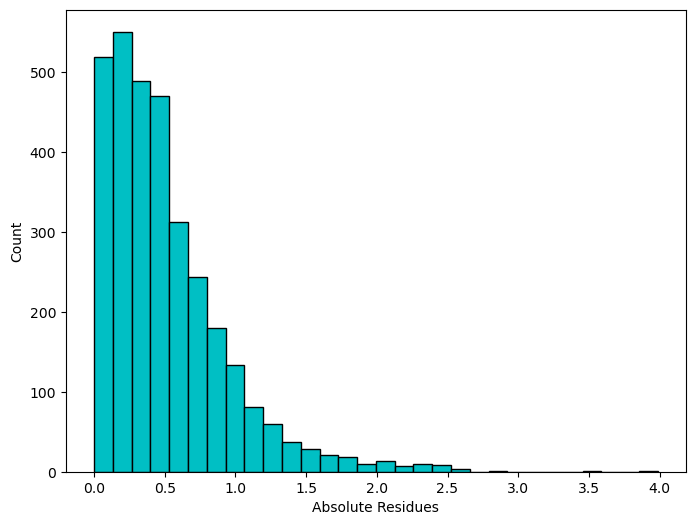
\includegraphics[width=14cm]{./assets/residues_histogram_ex1_PartII.png}
              \caption{The distribution of absolute residues for MLP regression on wine quality prediction using an histogram with 30 bins}
              \label{fig:PartII-ex1}
          \end{figure}

    \item \textbf{Since we are in the presence of a \textit{integer regression} task, a recommended trick is to
          round and bound estimates. Assess the impact of these operations on the MAE of the MLP learnt in the previous question.}

          \vskip 0.3cm
          \lstinputlisting[language=Python]{./assets/code_2.py}

          MAE without operations: 0.4937438468885914        \\
          MAE with rounded and bounded predictions: 0.43125

          \vskip 0.2cm
          By rounding to the nearest unit and bounding the estimates between 1 and 10 (as per the \textit{FAQ}), we get a lower Mean Absolute Error.
          The wine quality is an integer between 1 and 10, so it is expected that rounding and bounding the estimates gets them closer to the real integer values.

    \item \textbf{Similarly assess the impact on RMSE from replacing early stopping by a well-defined
          number of iterations in $\{20,50,100,200\}$ (where one iteration corresponds to a batch).}

           \vskip 0.3cm
          \lstinputlisting[language=Python]{./assets/code_3.py}

          RMSE with 20 iterations: 1.0336201651006487  \\
          RMSE with 50 iterations: 0.7060815422297181  \\
          RMSE with 100 iterations: 0.6641845695241441 \\
          RMSE with 200 iterations: 0.6393054830316605

    \item \textbf{Critically comment the results obtained in the previous question, hypothesizing at least
          one reason why early stopping favors and/or worsens performance.}

          \vskip 0.3cm
          Blah
\end{enumerate}
\end{document}
